\documentclass[prl,twocolumn,preprintnumbers,reprint]{revtex4}
\usepackage{amsmath,amssymb}


\usepackage{overpic,color}
\newcommand{\ud}{\,\emph{d}}
\newcommand{\dd}{\mathrm{d}}
\newcommand{\pp}{\partial}
\newcommand{\intn}{\!\!\int\!}
\newcommand{\bu}{{\bf u}}
\newcommand{\br}{{\bf r}}
\newcommand{\rd}{{\rm d}}
\newcommand{\be}{\begin{equation}}
\newcommand{\en}{\end{equation}}


\usepackage{amssymb}
\usepackage{amsmath}
\usepackage[T1]{fontenc}
\usepackage{amsfonts}
\usepackage{graphicx}% Include figure files
\usepackage{subfigure}
\usepackage{dcolumn}% Align table columns on decimal point
\usepackage{bm}% bold math
\usepackage{hyperref}
\usepackage{empheq}
\usepackage{natbib}
\usepackage{color}
\newcommand*{\citen}{}% generate error, if `\citen` is already in use
\DeclareRobustCommand*{\citen}[1]{%
  \begingroup
    \romannumeral-`\x % remove space at the beginning of \setcitestyle
    \setcitestyle{numbers}%
    \cite{#1}%
  \endgroup
}

\begin{document}
\preprint{Version 0.85}

\title{Geometrically frustrated, two-dimensional nematics confined by a rectangular box
}

\author{Xiaomei Yao and Hui Zhang$^*$}
\affiliation {School of Mathematical Sciences, Beijing Normal
University, Beijing 100875, P.R. China  }
\date{\today}

\author{Jeff Z. Y. Chen\footnote{Email: jeffchen@uwaterloo.ca}}
\affiliation{ Department of Physics and Astronomy, University of Waterloo, Waterloo, Ontario, Canada, N2L 3G1 }
\date{\today}

\begin{abstract} When an spatially homogeneous system that displays a nematic ordering on a two-dimensional surface is confined in a rectangular box, the nematic-director field develops inhomogeneous textures accompanied by orientational defect points because of the geometric frustrations. We provide the solutions to the extended Onsager model, which classify the nematic textures and defect patterns in terms of a few relevant, dimensionless geometric parameters. The previous experimental and theoretical findings related to this type of systems are critically examined in light of our new solutions, based on the determined free-energies of different defect states.
\end{abstract}

\maketitle

\clearpage
\newpage

Nature has it that some physical systems of vastly different scales and composed of different materials present the same phenomena that in-turn can be classified by a single physical picture. The topic of anisotropically shaped particles confined on a surface with a boundary  enclosing them is an excellent example. The word ``particles'' needs to be interpreted generally. These could be a thin layer of real liquid-crystal molecules confined in a micron-sized well \cite{Tsakonas2007}, aqueous suspensions of actin filaments \cite{Mulder2011} and linearly shaped virus \cite{Lewis2014} confined in a microchamber, and micron-sized colloidal silica rods\cite{Cortes2017} or visible-range granular rods \cite{Galanis2006,Galanis2010} flatly laid on a leveled bed confined by a box of approximately one order of magnitude larger.
In an ideal bulk state without a boundary, the anisotropic nature of these particles drives them into the formation of a directionally-ordered but spatially-homogeneous liquid state known as the nematic phase \cite{deG1993} under sufficiently high particle-number density. A uniform orientational direction, along the nematic director, can be identified.

The geometric confinement, however, disrupts the otherwise uniform, directionalized pattern. The frustrated direction field begins to display a range of different configurations and the orientational pattern now shows topological defects. Typical examples of these patterns are shown in Figs. \ref{P1} and \ref{P4} within the rectangular confinement. While understanding topological defects in liquid crystals is a research field that spans over other types of geometry  \cite{deG1993, trebin1982topology, kleman1989defects, Kleman2006, Alexander2012}, here we focus on two-dimensional (2D) systems with a simple rectangular confinement boundary. We demonstrate that these simple systems display essential features of the more complicated liquid-crystal confinement problems and that the orientational patterns observed in the above experiments can all be qualitatively accounted for by extending a fundamental statistical-physics model known as the Onsager theory \cite{Onsager1949}. % in 2D.**COMMENTS**

There are only three most relevant, dimensionless parameters that control the type of resulting nematic patterns in the model. The aspect ratio of a confining rectangle $b/a$, where $a$ and $b$ are the short- and long-side lengths,
and the box-rod size ratio  $a/L$, where $L$ is the length of a rodlike particle, define the confinement geometry.
In a system consisting of $n$ sterically repelling particles, the reduced number of particles per unit area,
$
L^2 \rho \equiv L^2 n/ab,
$ determines the degree of orientational ordering and hence the type of nematic patterns as well.
Originally, \citeauthor{Onsager1949} proposed a free-energy model for the bulk properties of the isotropic-nematic transition in three-dimension \cite{Onsager1949}. The model was later extended to include the positional-dependence of the distribution function \cite{McMullen88,Holyst88,McMullen1990,Chen1992,Chen1993,Koch1999,Roij01}. For the current problem, the free-energy must be minimized with the particle configurations, which produces a solution of the distribution function ${f}({x,y,\theta})$ for given $[L^2 \rho$, $a/L$, $a/b]$, where $x, y$ are the Cartesian coordinates to describe the location of a point in the box and $\theta$ is an angle to describe the particle's axial direction from the $x$-axis \cite{Chen2013}.

\begin{figure*}[!t]
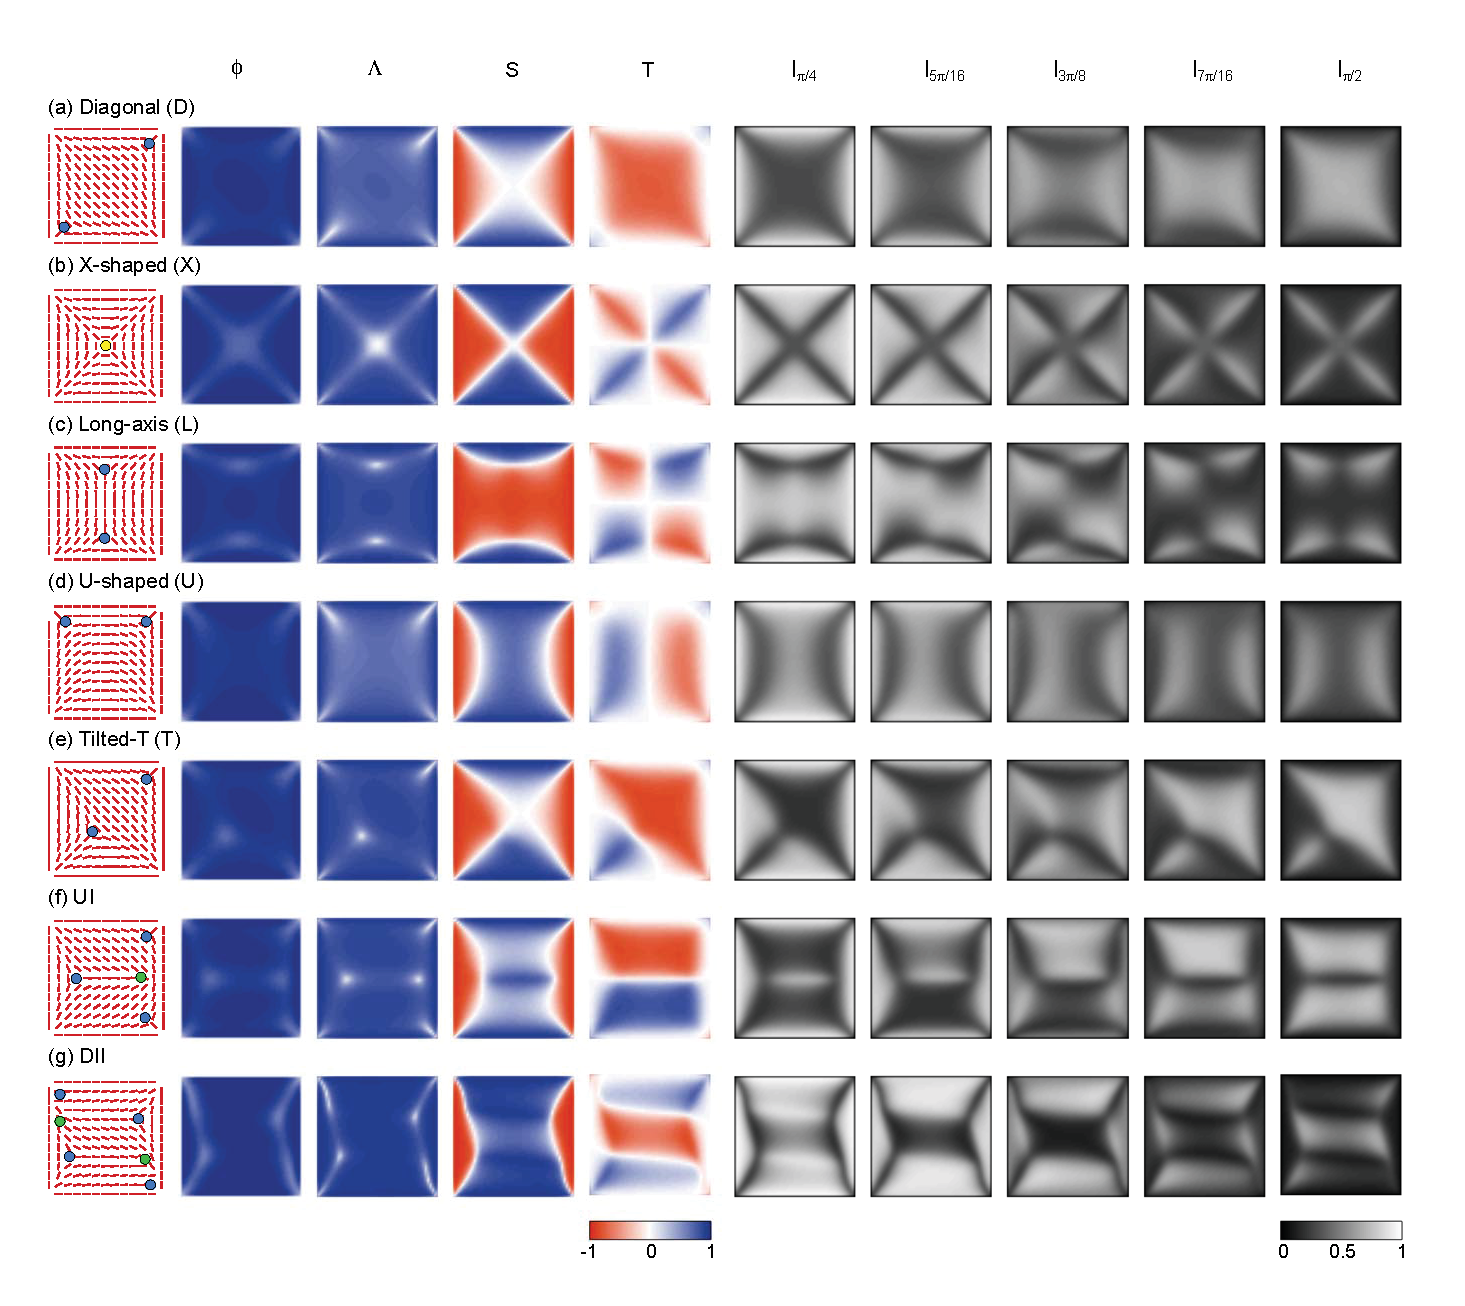
\includegraphics[width = 2.0 \columnwidth]{eps/s_t_phiCh.eps}
%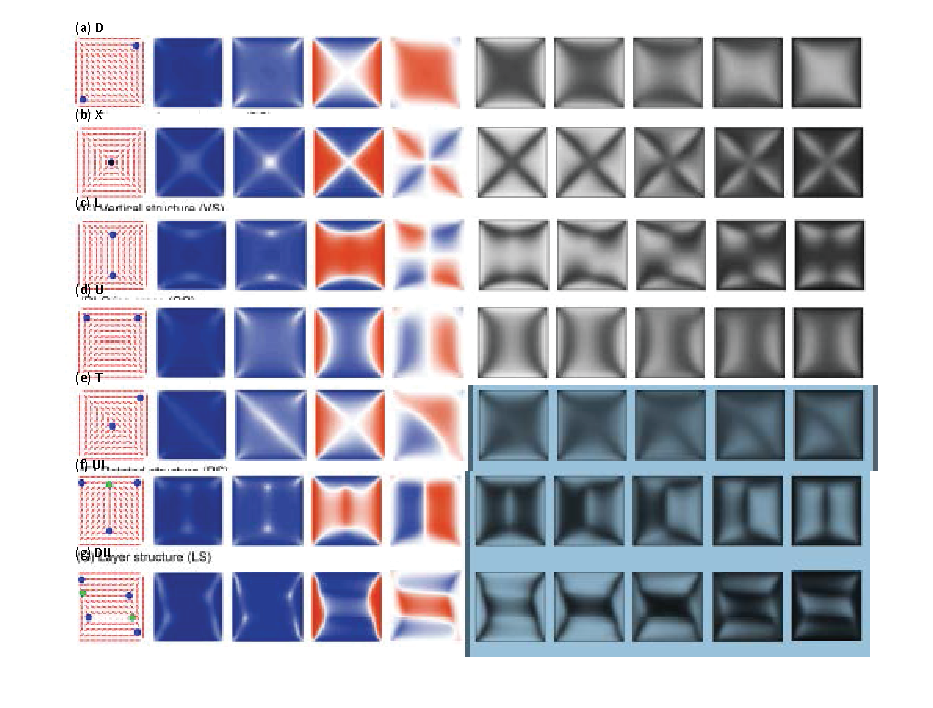
\includegraphics[width = 2\columnwidth]{eps/FIG1.eps}
\caption{Nematic defect structures found from the solutions to the extended Onsager model for $b/a=1$. Every structure is visualized by six methods: nematic-director field, fluid density variation $\phi$, main-axis orientational order parameter $\Lambda$, orientational order parameters measured from $x$- and $y$-directions, $S$ and $T$, and five grey-scale crossed-polarizer images calculated according to \eqref{Idef}
for $\alpha=\pi/4$, $5\pi/16$, $3\pi/8, $, $ 7\pi/16$, and $\pi/2$.
The reduced parameters used to produce these structures are: $[L^2 \rho_0, a/L]  = [6.5, 8.0]$, $[8.0, 10.0]$, $[8.0, 10.0]$, $[6.5, 10.0]$, $[6.5, 8.0]$, $[8.0, 10.0]$, and $[8.0, 10.0]$
for states that are labeled by (a) diagonal (D), *** X, VS, T, U, UI, and DII,
{respectively ****PLEASE Complete*** and add names to the figures.}
The color scale used for columns 2-5 is indicated by the red-blue color bar and the grey scale used for all $I_\alpha$ plots is indicated by the black-white grey bar. The blue [***REDUCE the intensity of your blue color in the firs column***], yellow, and green circles label the defect locations of $-1/2$, $-1$, and $+1/2$ winding numbers, respectively. The first three grey-scale images of D and U states closely match the real crossed-polarizer images of a liquid crystal confined in 80$\mu$m square cells, reported in Ref. \citen{Tsakonas2007}.}\label{P1}
\end{figure*}

\begin{figure*}[!t]\begin{center}
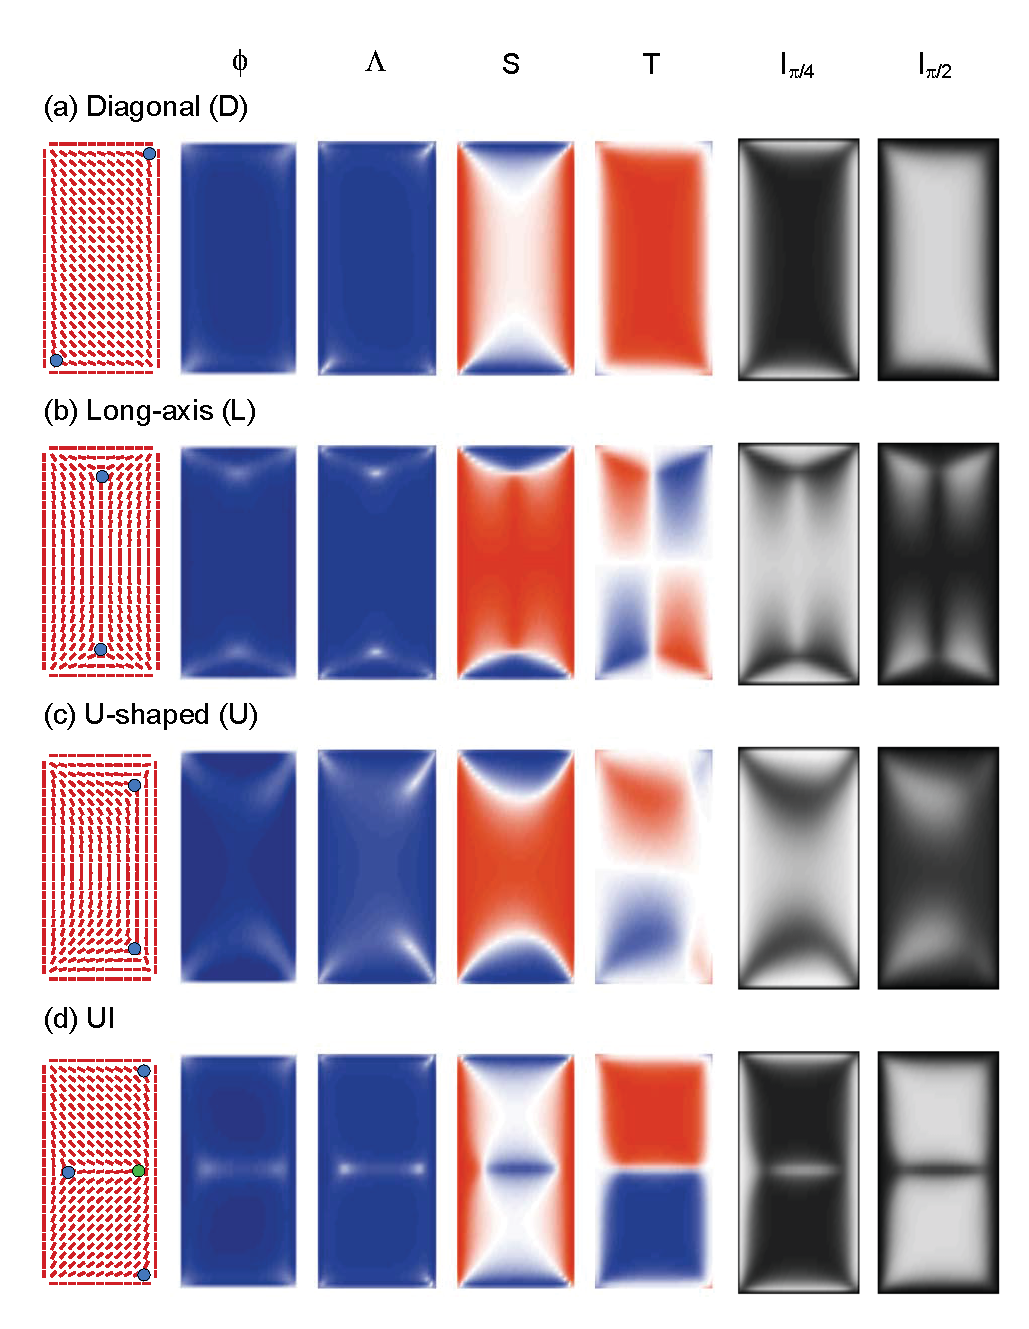
\includegraphics[width = 1\columnwidth]{eps/s_t_phi2Ch.eps}
%\includegraphics[scale=0.46]{eps/Tsa2.eps}
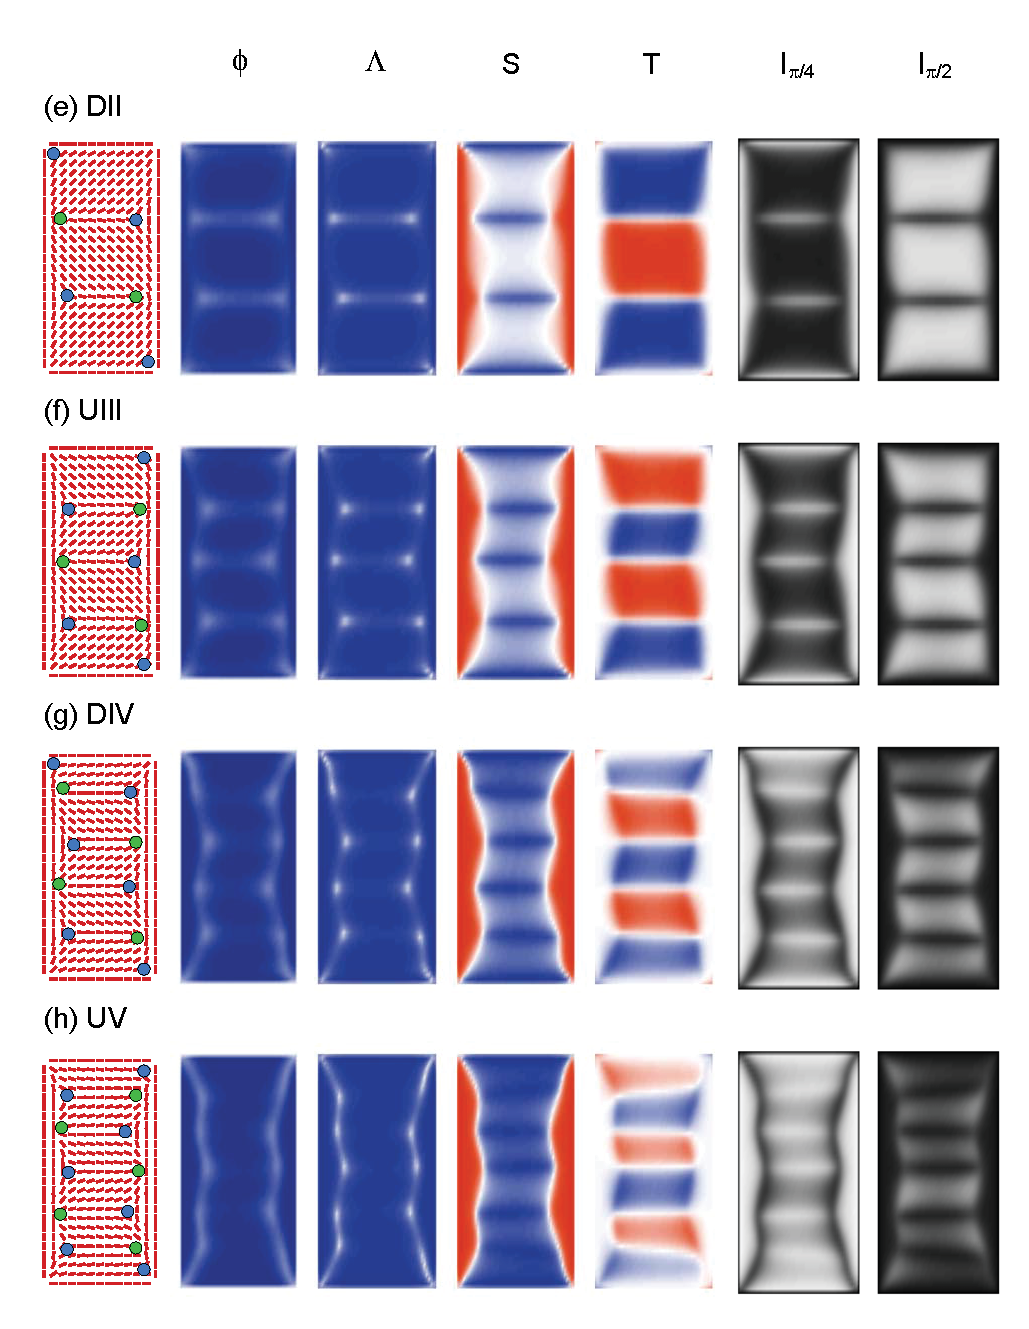
\includegraphics[width = 1\columnwidth]{eps/layer-stCh.eps}
%\includegraphics[scale=0.46]{eps/layer-Tsa.eps}
%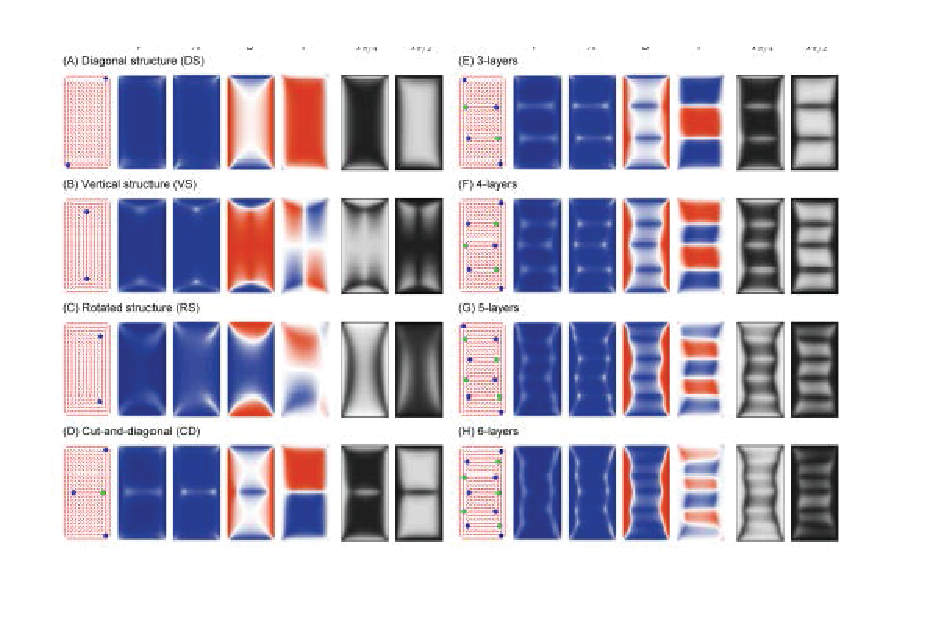
\includegraphics[width = 2 \columnwidth]{eps/FIG2.eps}
\caption{Nematic defect structures found from the solutions to the extended Onsager model for a rectangular box of aspect ratio $b/a=2$. Every structure is visualized by seven methods: nematic director field, nematic fluid density variation $\phi$, main-axis orientational order parameter $\Lambda$, orientational order parameters from the $x$- and $y$-axes, $S$ and $T$, and simulated crossed-polarizater images $I_{\pi/4}$ and $I_{\pi/2}$. The system parameters used to produce these structures are: $[L^2 \rho_0, a/L]  = [10.0, 7.5]$, $[10.0, 10.0]$, and $[8.0, 6.0]$, for (a)-(d), and $[10.0, 10.0]$ for (d)-(h). The color and grey scales and the meaning of colored circles are the same as in Fig. \ref{P1}.}\label{P4}
\end{center}\end{figure*}

Other theoretical tools have been used to study the current problem however the states are not identified completely. At the mean-field theory level, the Landau-de~Gennes model and the Oseen Frank model were used
to investigate the nematic patterns \cite{Tsakonas2007,Galanis2010,Luo2012,Lewis2014}; these models contain phenomenological parameters that cannot be easily identified with, for example, $a/L$ and $L^2\rho$. At a particle-based level,  Monte Carlo simulations were carried out to demonstrate the nematic patterns \cite{delasHeras2009,Dzubiella2000,Geigenfein2015,Mulder2015,Garlea2016}; they are not the best tool for calculating the free energy which is the key for identifying the phase diagram  .**COMMENTS** [**WHY take out GARLEA2016?**]

In a complex free-energy landscape, a single solution corresponds to a local (``metastable'') or global (``stable'') minimum.
%In this section we describe the structure of multiple defect states, both stable and metastable, found in this work.
The basic types of structures of stable and metastable states found in this work are visualized in Figs. \ref{P1} and \ref{P4} by various methods [the readers can refer to the supplementary material for the mathematical definitions]. An observed structure in a theoretical or real experimental system can correspond to the global minimum or can be trapped in a local minimum, if the free-energy barrier between these is high; our findings are discussed in comparison with others, illustrated in Fig. \ref{P12}. To place our model system in the nematic state, we let $L^2 \rho =10$ as an example and conduct our discussion of a phase diagram in terms of $a/b$ and $a/L$ as parameters, with illustrations of phase boundaries and metastable probabilities in Fig. \ref{Phase}.\\



\begin{figure*}[!t]\begin{center}
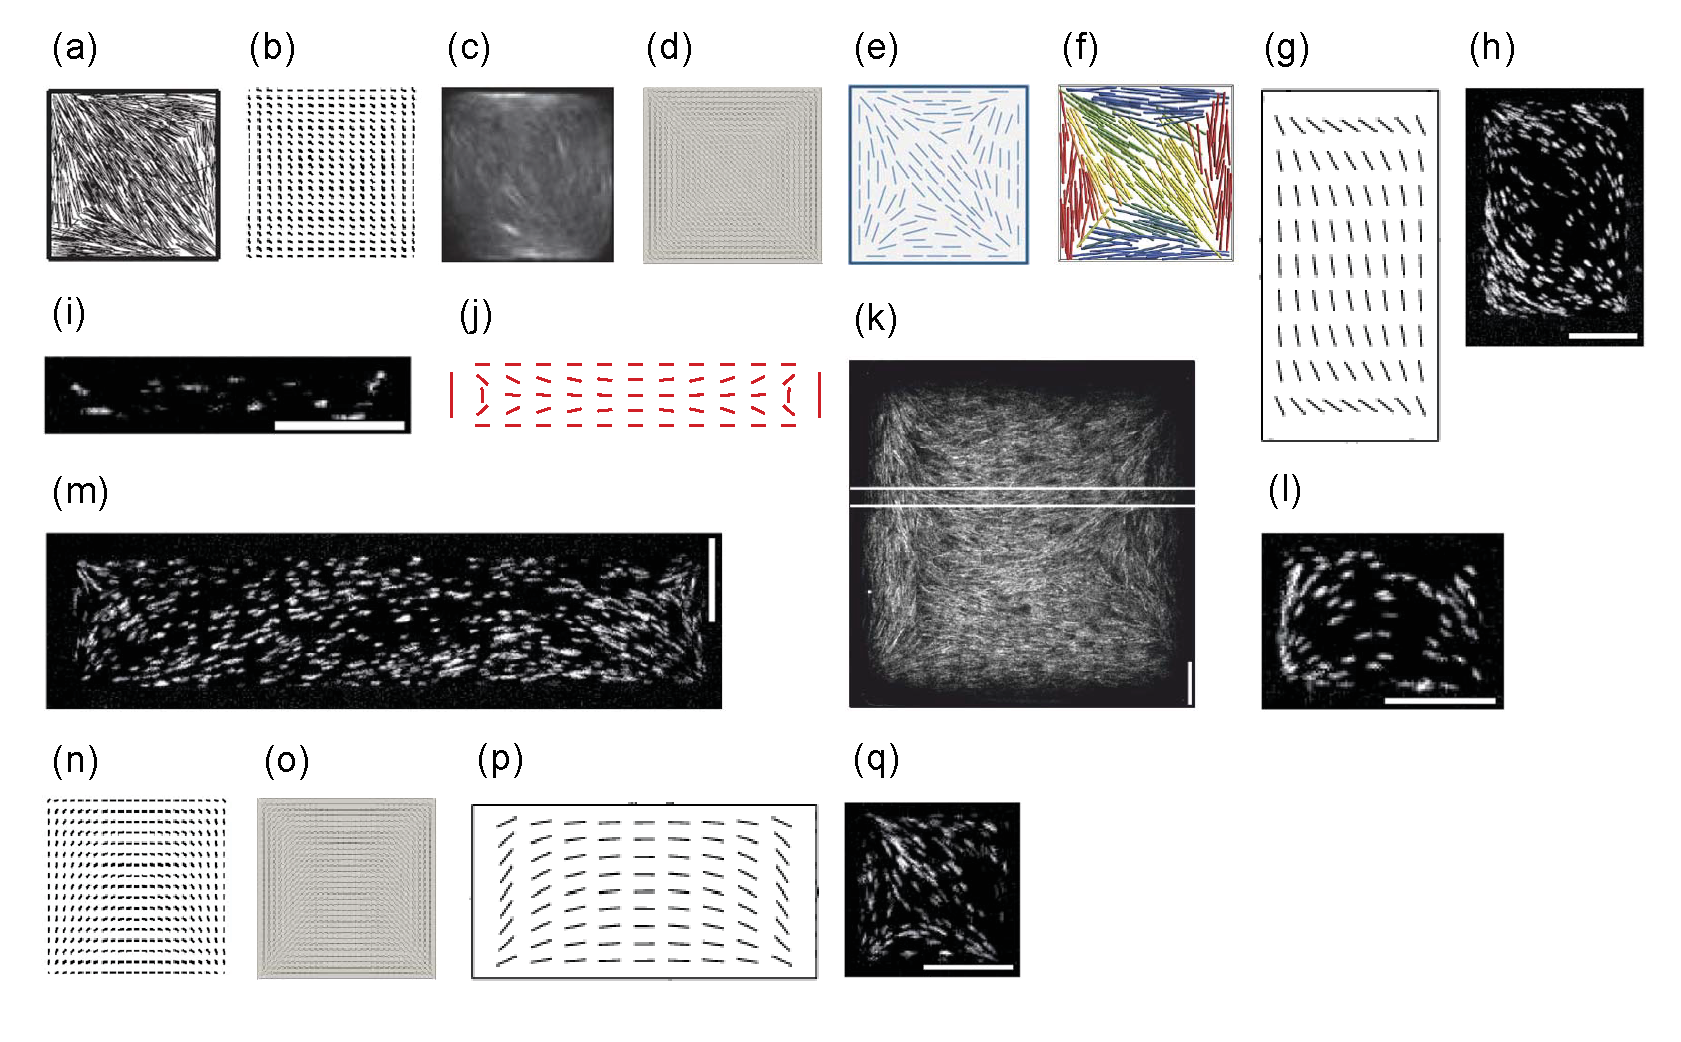
\includegraphics[width = 2\columnwidth]{eps/expCh.eps}
%\includegraphics[width = .32 \columnwidth]{eps/P1.eps}
\caption{Comparison to nematic textures found experimentally and theoretically.
These plots are adapted from: (a) Ref. \cite{Galanis2006} (experiment on granular rods); (b) and (n) Ref. \cite{Tsakonas2007} (solution to the LdG model);
(c) Ref. \cite{Mulder2011} (experiment on actin filaments); (d) and (o) Ref. \cite{Luo2012} (solution to LdG model); (e) Ref. \cite{Chen2013} (solution to the Onsager model); (f) Ref. \cite{Mulder2015} (MC simulations); (g) and (p) Ref. \cite{Lewis2014} (solution to the Oseen-Frank model); (h), (i), (l), (m), and (q) Ref. \cite{Lewis2014} (experiment on Y21M and {\it fd} viruses); as well as (k) Ref. \cite{Cortes2017} (experiment on colloidal rods). All plots were reproduced with consents from the original authors. Systems in (a)-(h) are in the D state, (i)-(k) L state, (l)-(p) U state, and (q) T state.
} \label{P12}
\end{center}\end{figure*}



\begin{figure*}[!t]\centering
\includegraphics[scale=0.295]{eps/P1.eps}
\includegraphics[scale=0.295]{eps/P2.eps}
\includegraphics[scale=0.295]{eps/P3.eps}
%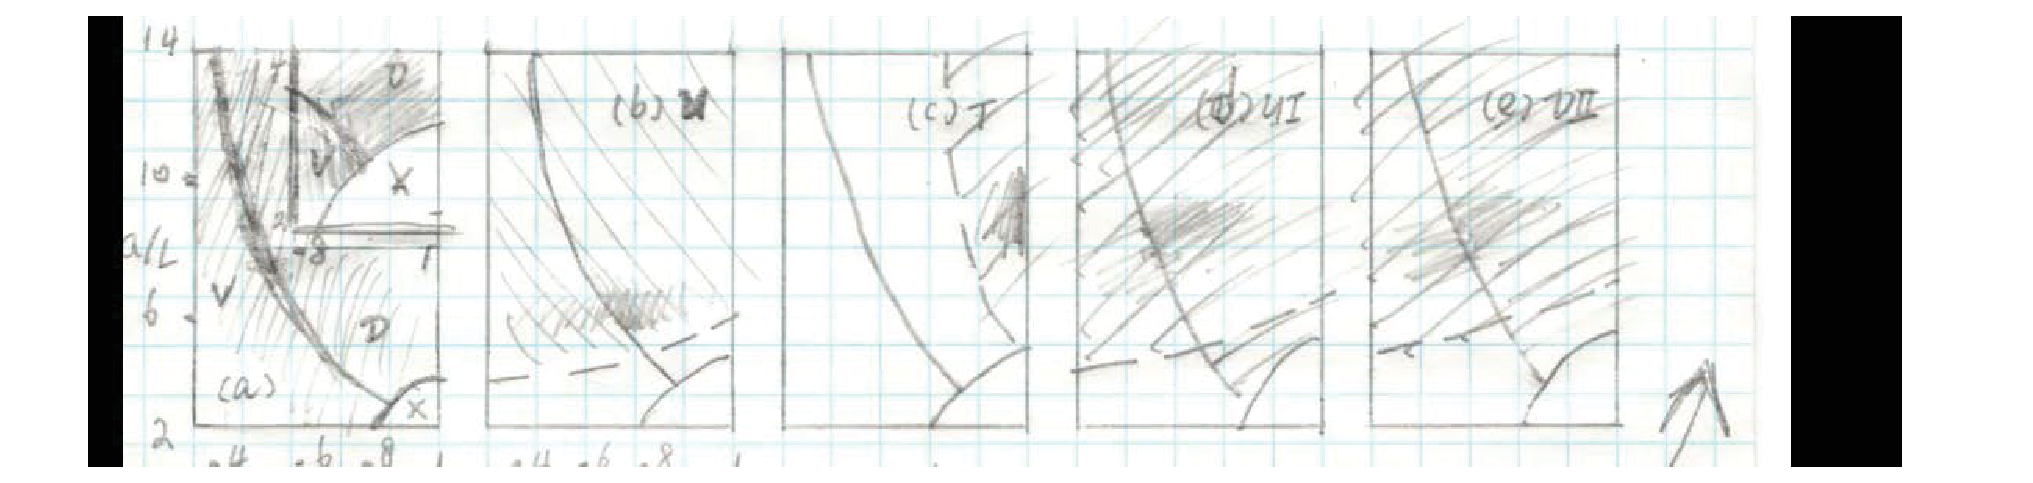
\includegraphics[width = 2\columnwidth]{eps/Phase.eps}
\caption{Phase diagram and relative probabilities for appearance of metastable states, $P$, in the nematic phase (for a given $L^2\rho = 10$). The solid phase boundaries in all plots divide D, V, and X states. The shaded areas in (b)-(e) are metastable regions of U, T, UI, and DII states, respectively. The color bars specify the relative probabilities, in comparison with those in states D  and V.} \label{Phase}
\end{figure*}




\noindent{\bf RESULTS AND DISCUSSION}

\noindent{\bf Nematic patterns.~} Here we classify the structures found from our work and categorize previously determined results.
The diagonal state (D), shown in Figs. \ref{P1}(a) and  \ref{P4}(a), is one of the most basic, and most studied defect patterns for all ratios of $a/L$. It has the lowest free energy over a large parameter space shown in Fig. \ref{Phase}(a), as the major body of the structure has a single nematic domain. \citeauthor{Galanis2006} described this nematic pattern in cm-long granular rods confined by a square cell of 29cm diagonal size, experimentally; the structure was visualized by their digital image \cite{Galanis2006}, reproduced here as Fig. \ref{P12}(a). \citeauthor{Tsakonas2007} reported the light transmission intensity observed by placing a real liquid crystal, E7 [***XIAOMEI CHECK the original ref**], in micron-sized square cells between crossed polarizers \cite{Tsakonas2007}. The light intensity images, $I_{\pi/ 4}$, $I_{5\pi/ 16}$, and  $I_{3\pi/ 8}$ constructed from our numerical results and displayed in Fig.~\ref{P1} are nearly identical to the experimental images, hence indirectly confirm that their observed state is D, a conclusion also supported by their own solutions to the Landau-de~Gennes model [see Fig. \ref{P12}(b)]. \citeauthor{Mulder2011} imaged the florescence filaments embedded in 6-$\mu$m long actin filaments  confined by a square cell of 30$\mu$m side length [Fig. \ref{P12}(c)], which also displays the same orientational pattern \cite{Mulder2011}. Theoretically, D is the common state that appears in the square-confinement solutions of the Landau-de~Gennes theory \cite{Tsakonas2007,Luo2012} and the extended Onsager theory
\cite{Chen2013},  the Monte Carlo simulations of rodlike particles in a slit with a square-boundary \cite{Mulder2015, Garlea2016}, **COMMENTS** and the rectangle-confinement solution of the Oseen-Frank theory \cite{Lewis2014}, reproduced here as Figs. \ref{P12}(b),(d)-(g), respectively.
The same D state has been observed in {\it fd}-virus confined in a flat rectangular box \citeauthor{Lewis2014} [Fig. \ref{P12}(h)].

In a system  with relatively smaller $a/L$, the boundary effects are more profound, influencing the structures in the box interior. When the box is nearly square ($b/a -1\lesssim 0.2$), a structure that keeps the four-sided symmetry of the original box, the X-shaped (X) pattern, is stable according to the inset of the phase diagram in Fig. \ref{P12}(b).
X has a single defect point at the center of the box and its main properties are illustrated by  Fig. \ref{P1}(b). It was deemed metastable previously from the preliminary solution of the extended Onsager model in a square box \cite{Chen2013}, however, is found here stable in a small parameter region.
Most experimental systems taken so far fall outside of this region; it would be useful to verify our prediction for the existence of the X-state experimentally.


Another stable structure where the symmetry is inherited from the boundary condition is the long-axis state, L, where the main domain of the nematic structure aligns with the long box-side direction, shown in Fig. \ref{P4}(b). It is one of the basic structures where a two-fold symmetry is maintained, naturally occurring for a system of large aspect ratio $b/a$, as described by the phase diagram in Fig. \ref{Phase}(a).
\citeauthor{Lewis2014} reported the existence of L in {\it fd}-virus confined
by a rectangle
with a large $b/a$, experimentally, showing an image of the dominating, long-axis nematics \cite{Lewis2014}[see Fig. \ref{P12}(i)]; they regarded that as a uniform nematic state but a careful examination of that image gives a hint of tilted nematic directions near the two ends of the narrow box; the image is similar to the director field produced from our solution shown in Fig. \ref{P12}(j) where the two defect points are located near the ends of the rectangular box, which were, with good probability, poorly captured by their experiment. Less intuitively, our solutions predict that L can be found, although metastable, for a confining square box $b/a=1$ [see Fig. \ref{P1}(c)], which was first conceptually suggested as a possibility without proof in Ref. \citen{Chen2013}. Coincidentally, using the Zwanzig model \cite{Zwanzig1963} (which over-simplifies a nematic structure by forcing rodlike particles to align only in the $x$- and $y$-directions, hence re-enders D impossible),
 \citeauthor{Pinto2013} illustrated an L-like state with two defect boundary curves \cite{Pinto2013}.
\citeauthor{Cortes2017} reported a confocal-microscopy nematic image of confined colloidal silica rods of 4 to 5 $\mu$m length in a $a/L=15$ square box [reproduced as Fig. \ref{P12}(k)]. According to Fig. \ref{Phase}(a), for a system of size $a/L \thicksim 15$,
the calculated metastable probability of L is low. On the other hand, their nematic state is clearly trapped in the L state with two defect points, similar to our illustration in Fig. \ref{P1}(c). It should be realized that starting from a dense, smectic-A state with the nematic director aligned along a box side, the L nematic state (not D) is a natural pathway to an isotropic state; although appearing with a low, natural probability,  because of the special initial condition, L can be energetically separated from the ground D state that requires a rotation of the main axis. This comes as concrete experimental validation of the existence of L in a $b/a=1$ system.


We find two other basic metastable structures in all parameter regions searched. The structure with a U-shaped (U) bending nematic domain [Figs. \ref{P1}(d) and \ref{P4}(c)] occupies almost the entire phase diagram, except for low $a/L$ region, as illustrated by the shaded area in Fig. \ref{Phase}(b). It has no rotational symmetry but contains a left-to-right mirror symmetry.
%The probability of finding U is relatively high near $a/L\sim 5$.
\citeauthor{Tsakonas2007} observed a typical image of U when they placed square wells filled with {E7} liquid crystald between crossed polarizers. Our simulated images, I$_{\pi/4}$, I$_{5\pi/16}$, and I$_{3\pi/8}$ in Fig. \ref{P1}(d) for U, are almost identical to the three plots in the middle column of their Fig. 2 \cite{Tsakonas2007}.
\citeauthor{Tsakonas2007} claimed that D and U are energetically degenerate. This cannot be the case, as the free energies associated with these two different patterns should be different; qualitatively, placing two same-signed defects at a shorter distance in U is bound to increase its free energy. The metastability of U was well-described by \citeauthor{Lewis2014} when they produced multiple virus systems confined by rectangles with various values of $a/L$ \cite{Lewis2014} [Fig. \ref{P12}(l) and (m)], experimentally. There is a close agreement between the probabilities of finding U assessed there and our Fig. \ref{Phase}(b).
Theoretically, U has been found in the square-confinement solutions of the Landau-de~Gennes theory \cite{Tsakonas2007,Luo2012} and the rectangle-confinement solution of the Oseen-Frank theory \cite{Lewis2014} [see reproduced Figs. \ref{P12}(n)-(p)].

Discovered for the first time in a theoretical calculation, we report here a tilted-T (T) state shown in Fig. \ref{P1}(e). It displays two nematic defect points, one close to the square center and the other on a diagonal line near a corner. The structure can be typically found in a near-square confining box, as illustrated in Fig. \ref{Phase}(c), due to the embedded symmetry.
Experimentally,  \citeauthor {Lewis2014} reported a nematic pattern that clearly resembles T [see reproduced Fig. \ref{P12}(q)], when they confined Y21M and {\it fd} viruses in a near-square box, which they identified as a variation of the D state \cite{Lewis2014}.\\

\noindent{\bf Defects and excited states.} From the general theory of nematic-defect structures \cite{Lubensky1992,Nelson2002a,Bowick2009,Turner2010} and according to the Poincar{\' e}-Hopf theorem, the total winding number as the summation of individual contributions,  must be the same for a given type of geometric frustrations \cite{do1976differential}.  The hard-wall boundary condition adopted in this work yields the tangential boundary condition (planar alignment), which enforces the main molecular axis to align in parallel to the confining wall surface perfectly \cite{Poniewierski1988,ChenCui1995}. As such, the total winding number of defect points appeared in each basic structure is $-1$, exactly following this theorem, as can be seen  from Figs. \ref{P1}(a)-(e) and \ref{P4}(a)-(c).

Our calculation shows that excited states beyond basic structures can be stablized, where pairs of $\pm 1/2$ defects are inserted into the basic defect patterns.
Among these are UI [Figs. \ref{P1}(f) and \ref{P4}(d)], UIII [\ref{P4}(f)], and UV [\ref{P4}(h)] where one, three, and five $\pm 1/2$ pairs show up in an otherwise U state, and DII [Figs. \ref{P1}(g) and \ref{P4}(e)] and
DIV [\ref{P4}(g)]  where two and four $\pm 1/2$ pairs show up in an otherwise D state. The insertion makes the structure
multi-layered.
Each layer has its own tilted, main nematic direction, altered layer by layer. These structures were found by enforcing the corresponding initial guesses in our solutions, which traps the system in these structures.
These metastable patterns can be created as long as the $b/a$ ratio can accommodate the space needed to sustain the layered structures.
As a general guideline, from our trials, we found that a maximum of three layers can be stabilized per unit $b/a$. Figures \ref{Phase}(d) and (e) demonstrate the region in phase space where UI and DII can be stabilized. No other experimental or theoretical study yields these excited states so far.

The interaction between nematic defects appearing on a surface can be compared with electrostatics {\cite{Lubensky1992,chaikin1995principles}}. Within this analogy, the defects with a positive (or negative) winding number play the role of positive (or negative) point-like
charges. Hence, the three repelling negative defects keep themselves as far as possible in UI and the positive defect finds itself a suitable balancing position inside the three negative defects to maximize the attractions it experiences.
These excited states can be viewed as insertion of (long) dipole pairs into an existing defect pattern. The alteration of the dipole axes are needed to maintain the electrostatic stability.

In some theoretical work, however, soft boundary conditions were used where the nematic layers at the boundaries are allowed to point at directions other than planer, with an energy penalty. One consequence is that the near-corner defects can resolve themselves to save the local defect-point free energy, in expense of increasing the energy penalty of the nearby, tilted boundary molecules \cite{Tsakonas2007,Luo2012,Lewis2014}. As such, the Poincar{\' e}-Hopf theorem can no longer be followed. As matter of fact, the nematic defects seem to have melted away at the rectangular corners of plots in Figs. \ref{P12}(b), (d), (g), and (n)-(p), which can be contrasted with the defects showing in our Figs. \ref{P1} and \ref{P4}. As well, the nematic defects in real experimental systems may not be always observed, if the defect points hide themselves near a corner of the confining rectangles or if the alignment at the boundaries are not perfectly planar. Assessment of those nematic textures with lesser number of defect points should be augmented with these melted defect points, to void over-classification and confusion.

Another important fact that must be noted is that the locations of the nematic defects can fluctuate to large extent, as shown by recent molecular simulations \cite{Humpert2017} and a real-time experimental movie of a colloidal liquid crystal \cite{Cortes2017}. The current study is  mean-field based and produces nematic patterns with particular symmetries. These symmetries may not always be visible in computer simulations or real experiments  with fluctuating defect points.\\

\noindent {\bf METHODS}

\noindent{\bf Extended Onsager model.} Of the central focus is the density distribution function $\rho(\br,\bu)$ which characterizes the probability density of finding the centers-of-mass of the rodlike molecules at a spatial position specified by the vector $\br$ with the condition that the rods are pointing at the direction specified by a unit vector $\bu$. Here we assume that $\rho(\br,\bu)$ is normalized to $n$.
%\begin{equation}\label{rhonorm}
%\intn\intn\rho(\br,\bu) \dd \br \dd \bu = n.
%\end{equation}
For a given, unknown distribution $\rho(\br,\bu)$, accurate to the second-virial coefficient, the extended Onsager model states that the free energy of the system is a functional,
\begin{equation}
\begin{aligned}
\label{Fdef}
 \beta &F=\intn\rho(\mathbf{r},\mathbf{u}) \ln [L^2\rho(\mathbf{r},\mathbf{u}) ] {\rm d}\mathbf{r} {\rm d}\mathbf{u}\\
%&+\int \varrho(\mathbf{r},\mathbf{u}) \beta V(  \mathbf{r},\mathbf{u}  )  \;\dd\mathbf{r} \dd\mathbf{u}\\
&+ \frac{1}{2}\int\rho(\mathbf{r},\mathbf{u}) w(\mathbf{r},\mathbf{u};\mathbf{r}^\prime, \mathbf{u}^\prime)\rho(\mathbf{r}^\prime, \mathbf{u}^\prime)
%\;\dd\mathbf{r} \dd\mathbf{u} \dd\mathbf{r}^\prime \dd\mathbf{u}^\prime,
\end{aligned}
\end{equation}
where $\beta = 1/k_B T$, with $k_B$ being the Boltzmann constant and $T$ the temperature. To obtain the stable or metastable configurational properties, the free-energy  is to be minimized with respect to $\rho(\br,\bu)$ with the appropriate hard-wall boundary conditions. The free energy includes two terms. The first term is ideal-gas-like, containing both translational and orientational entropies of a spatially inhomogeneous and orientationally ordered gas of rodlike molecules. The kernal function $w(\mathbf{r},\mathbf{u};\mathbf{r}^\prime, \mathbf{u}^\prime)$ in the second term describes the interaction between two rods respectively having the coordinates $(\mathbf{r},\mathbf{u})$ and $(\mathbf{r}^\prime, \mathbf{u}^\prime)$. The two terms compete with each other as one prefers isotropic state and the other nematic state. The actual free-energy minimization procedure was carried out by using the mathematically equivalent self-consistent field theory
\cite{Chen2013, Chen2016}.
\\


%The free energy includes two terms. The first term is ideal-gas-like, containing both translational and orientational entropies of a spatially inhomogeneous and orientationally ordered gas of rodlike molecules. The kernal function $w(\mathbf{r},\mathbf{u};\mathbf{r}^\prime, \mathbf{u}^\prime)$ in the second term describes the interaction between two rods respectively having the coordinates $(\mathbf{r},\mathbf{u})$ and $(\mathbf{r}^\prime, \mathbf{u}^\prime)$. For excluded-volume interactions only, the Mayer expansion allows us to specify this function: $w=1$ if any parts of the two rods overlap and $w=0$ otherwise, similar to the treatment of an athermal non-ideal gas system.\cite{pathriastatistical} This, however, makes the kernal term {\emph {nonlocal}}, as one needs to specify the intersection point of two rods by extending two lines from the centers $\br$ and $\br^\prime$ in the directions of $\bu$ and $\bu^\prime$. Mathematical details are described in Appendix B.


\noindent{\bf Visualization.} Most experimentally accessible measurements of a 2D system, either through the crossed-polarizer imagining \cite{Tkachenko1995} or direct optical picturing \cite{Galanis2006,Mulder2011,Lewis2014,Cortes2017},  probe the physical properties of the distribution function of segments on a rodlike molecule.
This distribution can be deduced from $\rho(\br,\bu)$ by a mathematical identify. On the basis of that information, we can determine the local molecular density fraction $\phi(x,y)$, the local main-axis orientational parameter $\Lambda(x,y)$, the orientational order parameters in $x$- and $y$-directions $S(x,y)$ and $T(x,y)$, and simulate the light intensity variation when a 2D nematic cell is placed in a crossed polarizer with the first polarizer-axis making an angle $\alpha$ from the $x$-axis,
\begin{equation}\label{Idef}
I_\alpha(x,y) = {1\over 4}\left< [\sin(2\theta-2\alpha)]^2 \right >.
\end{equation}
The average is performed locally with respect to the molecular orientation $\theta$.\\

\noindent{\bf Data availability.} All step-by-step information on the definition of the visualized properties,  as well as theoretical and numerical methods are contained in the supplementary information.\\




%\begin{figure}[!t]\centering
%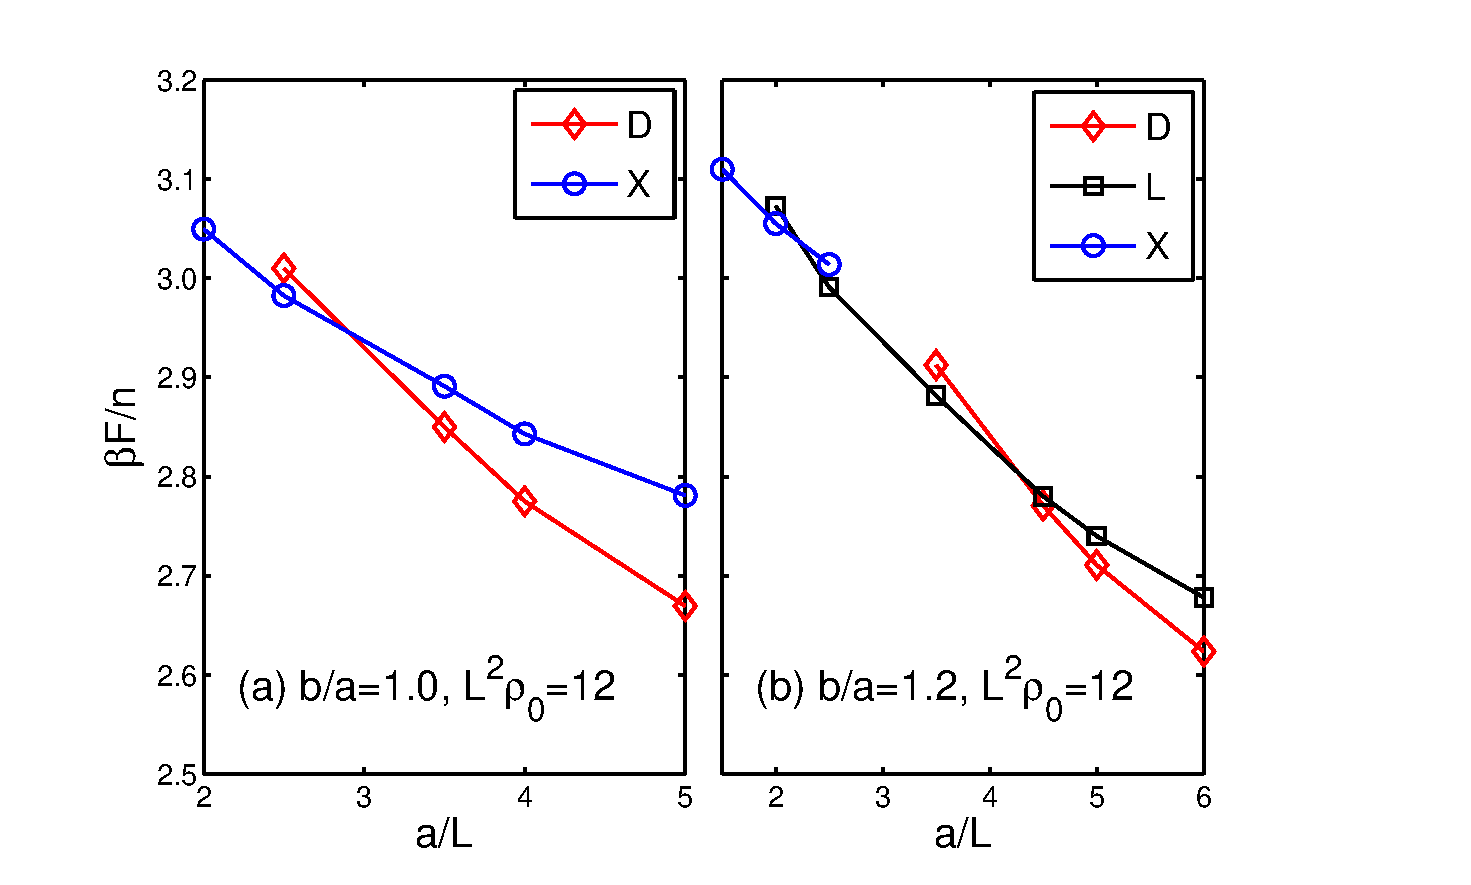
\includegraphics[width = 1.2 \columnwidth]{eps/energy-plot.eps}
%\caption{Two examples of the free-energy minima data as functions of $a/L$ for fixed (A) $[b/a, L^\rho_0]= [1,12]$ and (B)$ [1.2, 12]$. The crossing of these branches yields a phase boundary for the transition between the two involved states, of the first-order characteristics. } \label{P2}
%\end{figure}

%\begin{figure}[!t]
%\includegraphics[width = 0.85 \columnwidth]{eps/ABCD.eps}
%\caption{Phase diagrams for four given aspect ratios, plots (A)-(D) for $b/a=1, 1.2, 2, 3$, in terms of $a/L$ and $L^2\rho_0$. Refer to Figs. \ref{P1} and \ref{P4} for the defect structures that correspond to the labels of the stability regimes. A second-order phase transition curve (dashed) saparates the parameter space into ordered and isotropic (ISO) states.} \label{phase}
%\end{figure}


\noindent{\bf CONCLUSIONS}

In summary, we examine the 2D nematic-defect structures of rodlike molecules confined in rectangular box of various sizes and aspect ratios, using an extended version of the classical Onsager model for lyotropic liquid crystal systems. The main conclusions are based on numerical solutions to the model, which display a variety of basic and excited defect patters, all topologically different.
%Only two of these structures were examined in a preliminary study of the same theoretical model.
All optical images of real experimental systems taken in recent years are now systematically accounted for by our theoretical results. In addition, some structures are predicted for the first time in this work and should be verifiable in further experimental work.
The phenomena described here land on a number of branches in physics, materials science, and mathematics, forming problems of fundamental importance.


%Real liquid crystal fluids in a confined 2D cell of micron size, in which $a/L\gg 1$, is one of the ideal systems to experimentally study some of the defect patterns suggested. To complete our analysis, here we present simulated crossed-polarizer images of the seven structures in Fig.~\ref{P1}, as the polarizer axes rotate from $\alpha=\pi/4$ to $\pi/2$, according to \eqref{Idef}. To demonstrate the accuracy of these calculated images, the first three images (from $\alpha=\pi/4$ to $3\pi/8$) of DS and RS closely match the experimental results, shown in Fig. 2 of Ref. \citen{Tsakonas2007}. It is worth noting that the third images (for $\alpha=3\pi/8$) of DS and RS have an apparent up-down symmetry (phrased according to our orientational arrangement of the figures), which actually do not exist in fine details. There is no reason, on the basis of a general symmetry analysis of both DS and RS textures, that $I_{3\pi/8}(x,y)$ has this symmetry. This is not the view taken by authors of Ref. \citen{Tsakonas2007}. Not only they claimed that their experimental images have this symmetry, but they also produced similar images according to a solution of the Landau-de Gennes {\sf Q}-tensor theory. This discrepancy can be addressed by realizing the following. A careful study reveals that near the isotropic-nematic transition point, the position variation of the nematic state can be described by the primitive waves in a Fourier transforation, which show this symmetry. Any further harmonic waves in the Fourier series for the position variation at a deeper nematic state, however, destroy the symmetry.

We have left behind the thread of other theoretical issues such as whether there is indeed a long-range order
in a two-dimensional system \cite{Frenkel1985,Dijkstra2003} and whether or not
a density functional theory \cite{delasHeras2009} can repair the underestimate of the isotropic-nematic transition point from the Onsager model in 2D. The current work  demonstrates the beauty and triumphs of a simple fundamental physical idea considered by \citeauthor{Onsager1949} nearly 70 years ago --- the directional ordering seen in nematics can be captured by the needs to increase the orientational entropy and to decrease the excluded-volume interaction. While this consideration was proposed to deal with the bulk isotropic-nematic transition, adding geometric frustrations gives the model a new life. It can be used to study the nematics of rigid molecules embedded on the spherical surface
where the topological frustrations of accommodating a (headless) vector nematic field on a (curved) closed surface
produces multiple nematic defect states \cite{Wuyang2012prl,Wuyang2012pre,Liang2014}. It can also be used to study the 2D nematics of rigid molecules frustrated by confining geometry of various shapes: rectangle (this work and Ref. \citen{Chen2013}) and circle (Ref. \citen{Chen2013}).





%\renewcommand\refname{Notes and references}
%\bibliography{Ref2}
\bibliography{Ref2,jy,LCC,yao,RefYSW} %You need to replace "rsc" on this line with the name of your .bib file

%\begin{thebibliography}{99}
%\end{thebibliography}
\bibliographystyle{apsrev4-1}
%\bibliographystyle{unsrt}
%theme:
%	plain: sort alphabetically based on author, year and title.
%	abbrv: abbreviation of plain style
% 	unsrt: sort based on the order of citation

%\onecolumngrid

%\vfill
%\newpage


\end{document}
































